\chapter{流形及其张量场}\label{appx:manifold}
    \begin{figure}[h!]\centering
    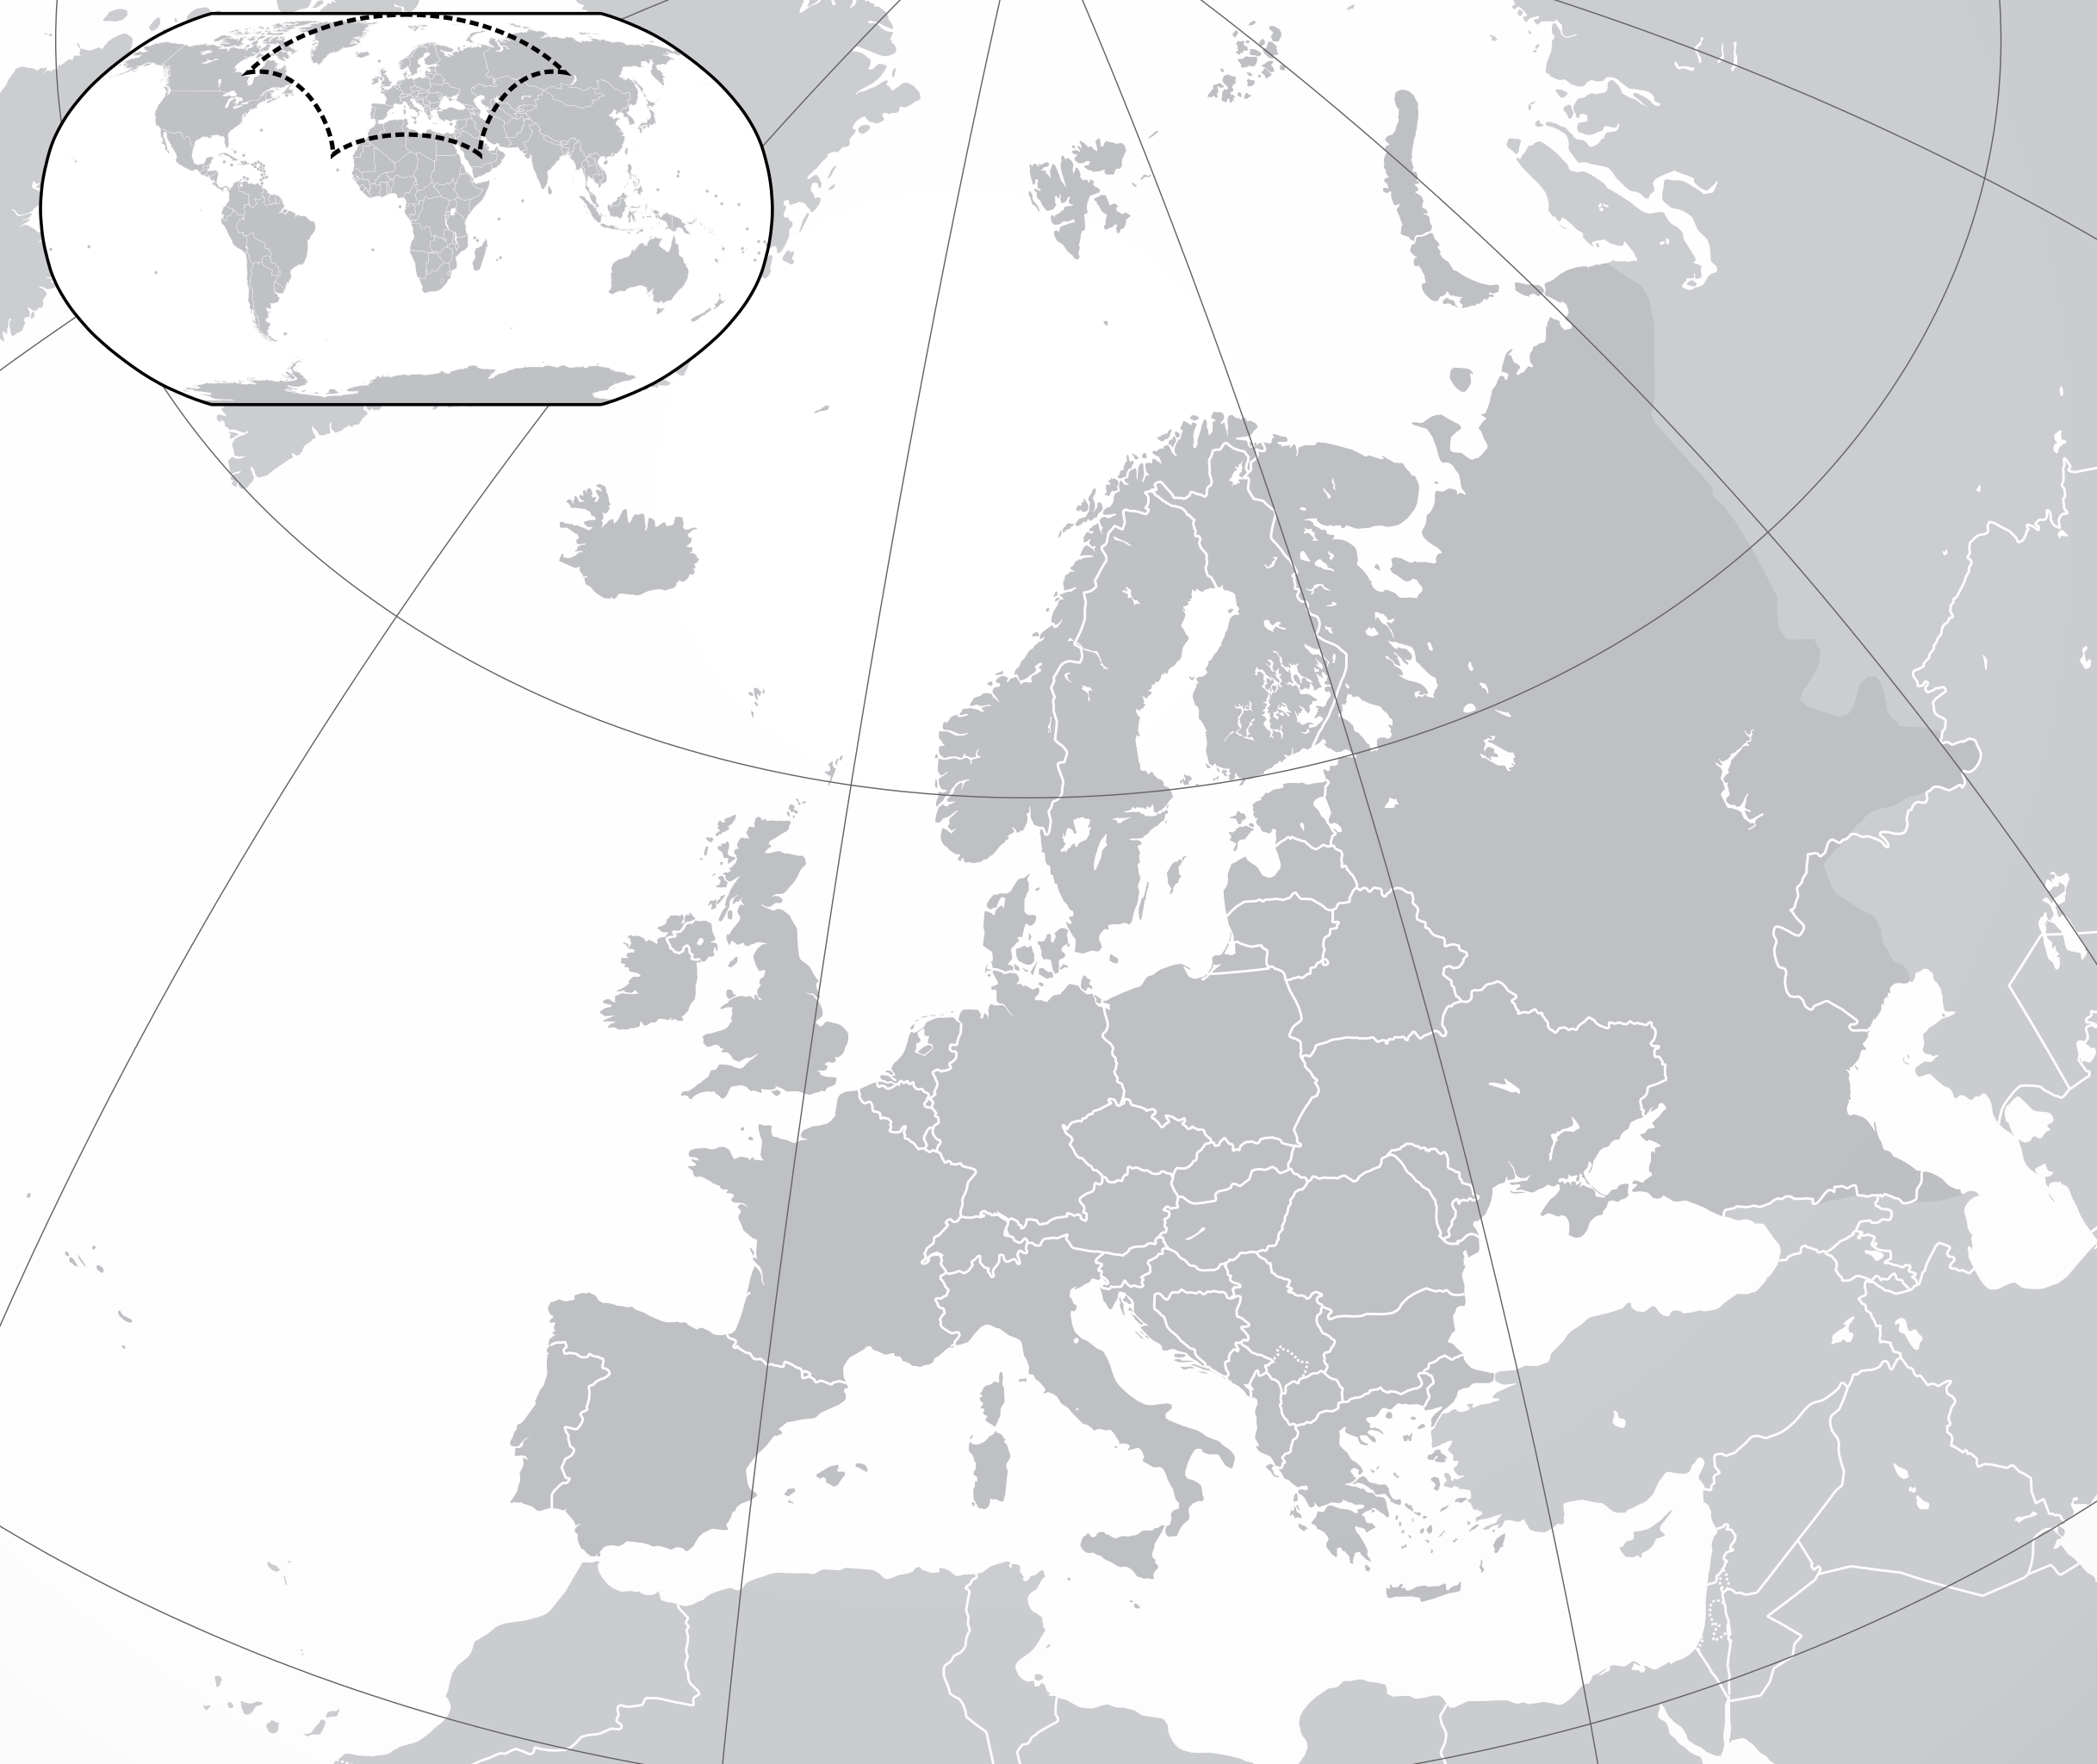
\includegraphics[width=.8\textwidth]{fig/appx/Europe-Blank.png}
    \caption{地球的局部坐标网格,图示为欧洲}
\end{figure}

\section{实流形}
物理背景作为拓扑空间,是无特征且无定形的,其中的点和曲线是不能先验识别或定义的,除非利用坐标系。有用的背景从来不可能真正脱离坐标。
坐标方法就是一种给背景点连续指定 $\R^n$ 数据的映射。
例如,平面上附着不同的坐标空间,一种可存放正交坐标,一种可存放极坐标,从而可赋予某点 $p$ 正交坐标 $(0,1)$,也可赋予极坐标 $(1,\pi/2)$,如图 \ref{fig:coor-chan}。拓扑学的同胚关系可描述坐标的指定,因为同胚具有双向连续性,且两个点不会被分配到同一坐标,从而避免歧义。
当然,同胚使得许多坐标系能力有限,不能揽下全局。比如,极坐标系不能完整覆盖 $\R^2$,坐标取值为 $V=(0,+\infty)\times(0,2\pi)$。因此常考察开子集。为圆满完成指派任务,整个背景须由若干坐标系拼接,且互相分担对方力所不及之地。

\begin{definition}
    置 $(M,\mathscr T)$。存在 $n\in\N$,使 $M$ 任意点都存在邻域同胚于 $(\R^n,\mathscr T_u)$ 某开集,则称其\textbf{局部欧的}。
    显然等价说法为:$\exists$ $M$ 的开覆盖 $\mathscr P$ 使 $\forall O\in\mathscr P$,$\exists$ 同胚 $\psi:O\to V\in\mathscr T_u$。
    $\psi$ 称为\textbf{坐标映射},$\psi(p)$ 称为 $p$ 的\textbf{坐标}。$O$ 称为\textbf{坐标域}(patch),$(O,\psi)$ 称为\textbf{坐标系}或\textbf{图}(chart)。$\mathscr P$ 所相应的坐标系族 $\mathcal A=\{(O,\psi)\}$ 称为\textbf{图册}(atlas)。$(M,\mathcal A)$ 称为\textbf{局部欧氏空间}。维数为 $\dim M:=n$。当 $\mathcal A$ 自明时简记 $M$。
\end{definition}

\begin{remark}
    同胚连续性由全集拓扑或诱导拓扑衡量。原则上可修改定义,使其允许各坐标系不同维,这样空间无唯一维数,但实用价值不大。
\end{remark}

同胚赋予的第 $i$ 个坐标构成映射 $x^i:O\to\R$,坐标系又常记 $\{x\}$。
就某个坐标系而言,坐标域的子集
    $\{p\in O: x^i(p)$ 是常函数,$i=2,\cdots,n\}$
可看成以 $x^1$ 为参数的路径,称其是一条 $x^1$ \textbf{坐标线}(coordinate line)。其它情况以此类推。全体坐标线构成\textbf{坐标网格}。
坐标域是某点邻域,故坐标系又称局部坐标系,同胚又称局部同胚。仅用一个坐标域就能覆盖则称\textbf{平凡的}(trivial),此时可称坐标系是整体坐标系。典型的例子是 $\R^n$ 自身。设 $a=(x^1_a,\cdots,x^n_a)\in\R^n$,恒等映射给出\textbf{自然坐标} $\psi(a)=(x^1(a),\cdots,x^n(a))=a$。

\begin{definition}
    第二可数 $T_2$ 的局部欧氏空间称为 \textbf{$n$ 维实拓扑流形},简记\textbf{拓扑流形} $M$。部分教材还加上仿紧的条件。将 $\R^n$ 换为 $\C^n$ 就是\textbf{复流形}。
\end{definition}

\begin{figure}[ht]
    \centering
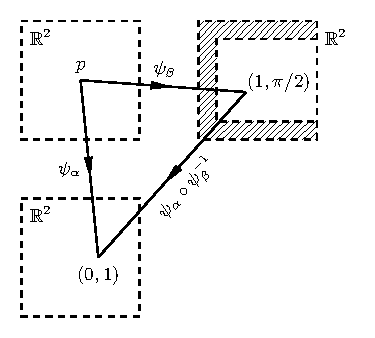
\includegraphics[width=.4\textwidth]{fig/appx/coor-chan.pdf}
    \caption{坐标变换}\label{fig:coor-chan}
\end{figure}

由于坐标域都是开的,故必存在相交之地。此处便涉及坐标系的转化。

\begin{definition}
    置某个图册 $\mathcal A$。
    取 $(O_\alpha,\psi_\alpha),(O_\beta,\psi_\beta)\in \mathcal A$ 满足 $O_\alpha\cap O_\beta\ne\mt$。
    若 $\psi_\alpha\circ\psi_\beta^{-1}$ 的 $r$ 阶导函数连续($C^r$ 性),则称它们是 $C^r$\textbf{-相容的}。$\psi_\alpha\circ\psi_\beta^{-1}$ 称为\textbf{坐标变换}或\textbf{转移函数}。
    若相交坐标系皆 $C^r$-相容,则 $\mathcal A$ 称为 $C^r$\textbf{-图册}。$C^\infty$-相容称为\textbf{光滑相容}或\textbf{相容}。
\end{definition}

\begin{remark}
    坐标变换可显式地表为 $n$ 个 $n$ 元函数,其 $C^r$ 性由 $\R^n$ 分析学给出。
\end{remark}

假设有两个图册 $\mathcal A,\mathcal B$。它们可能并不相容,即其间存在相交但不相容的坐标系。如果它们相容,则可合并为一个更大的图册。当然希望将所有相容的坐标系都囊括进来,尽可能构成足够大的图册。

\begin{definition}
    不真含于任何 $C^r$-图册的 $C^r$-图册称为\textbf{最大的}(maximal) 。若局部欧氏空间 $(M,\mathcal A)$ 的图册 $\mathcal A$ 是 $C^r$-最大图册,则称 \textbf{$C^r$-实微分流形},简称 $C^r$-流形。常考虑光滑流形。对复流形而言即要求微分结构全纯(解析)。
    最大图册又称\textbf{微分结构}。
\end{definition}

\begin{remark}
    拓扑流形是第二可数 $T_2$ 的 $C^0$-流形。实际上常默认微分流形定义中的局部欧氏空间为拓扑流形,甚至补充仿紧等性质。
\end{remark}

\begin{eg}
    \textbf{通常流形}就是指 $(\R^n,\mathscr T_u)$ 赋以包含自然坐标系的最大光滑图册。
\end{eg}

\begin{definition}
    置 $C^k$-流形上的曲线 $C$。若 $\forall p\in \Im C$,存在坐标系 $(\psi,O)$ 使 $p\in O$ 且\textbf{参数方程} $\psi\circ C$ 是 $C^r$ 的($r\leqslant k$),就称 $C$ 是 $C^r$\textbf{-曲线}。有限个光滑曲线收尾相连构成\textbf{分段光滑曲线}。
\end{definition}

\begin{remark}
    $r\leqslant k$ 使曲线 $C^r$ 性与坐标选择无关。此后类似概念的良定义性均同理。
\end{remark}

\begin{theorem}
    流形上,路径连通 $\iff$ 连通
\end{theorem}

\begin{figure}[ht]
    \centering
    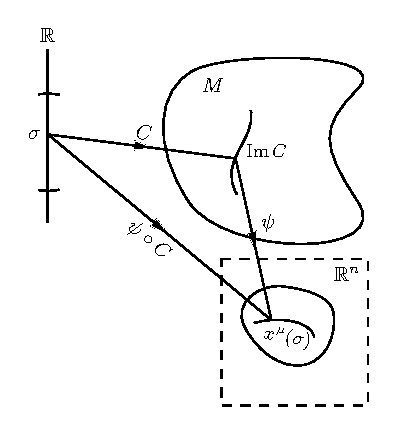
\includegraphics[width=.4\textwidth]{fig/appx/curve.pdf}
    \caption{曲线}
\end{figure}

\begin{definition}
    置 $C^k$-流形 $M,M'$。$f:M\to M'$ 称为 $C^r$\textbf{-映射},若 $\forall p\in M$,存在坐标系 $(\psi,O),(\psi',O')$ 使 $p\in O,f(p)\in O'$ 且 $\psi'\circ f\circ \psi^{-1}$ 是 $C^r$ 的($r\leqslant k$)。
    \textbf{$C^r$-微分同胚}(diffeomorphism)是双向 $C^r$ 的双射。光滑同胚的流形一定程度上可视作相等的,故又称\textbf{自同胚}。
\end{definition}
\begin{remark}
    固然希望抽象地定义 $f$,但准确定义又总要使用坐标系,通过 $\psi'\circ f\circ \psi^{-1}$ 来确定 $f$。
\end{remark}

以光滑流形为对象、光滑映射为态射,构成\textbf{光滑流形范畴} $\cate{Man}$,同构态射即光滑同胚。

考察光滑映射 $\phi:M\to N$。在 $p,\phi(p)$ 分别取坐标系 $\psi,\psi_N$,则 $\phi$ 可借助坐标系表为 $\psi_N \circ\phi\circ\psi^{-1}$。
倘若 $\phi$ 是同胚,则可定义新坐标系 $\psi':=\psi_N\circ\phi$,也即将 $\phi(p)$ 的坐标 $\psi_N(\phi(p))$ 视作 $p$ 的新坐标 $\psi'(p)$。这样给定一个 $\phi$ 相当于给定坐标变换 $\psi' \circ\psi^{-1}$。此即光滑同胚的主动、被动观点之别。

\begin{definition}
    置 $M$ 上的开覆盖 $\mathscr P=\{O_i\}$。若函数族 $\{\rho_i\}$ 满足
    \begin{itemize}
        \item $0\leqslant\rho_i\leqslant 1$;
        \item $\rho_i$ 在 $O_i$ 上光滑,且支撑在 $O_i$ 上:$x\notin O_i$ 时 $\rho_i=0$;
        \item $\sum_i \rho_i=1$,
    \end{itemize}
    则称为 $\mathscr P$ 的一个\textbf{单位分解}(partition of unity)。
\end{definition}
\begin{theorem}
    任何开覆盖均存在从属于它的单位分解。
\end{theorem}
\begin{proof}
    利用第二可数性。
\end{proof}

\section{切空间}

\begin{definition}
    流形上的函数称为\textbf{标量场}(scalar field)。置光滑流形 $M$,$U\subset M$ 上全体 $C^r$-标量场构成的集合记作 $C^r(U)$。常考虑实光滑函数。
\end{definition}

我们曾谈到矢量需要一个抽象定义。物理学的矢量总是靠作差或求导来产生,即切矢。因此可将切矢对应到曲线来定义。
给定一条穿过 $p\in M$ 的曲线 $\gamma$,要求其在 $p=\gamma(0)$ 处可导,规定给出相同切矢的曲线等价。相同性通过坐标分量($\psi\circ\gamma$ 在 $t=0$ 处导数)来判断。等价类 $[\gamma]$ 称为一个切矢。
Cartan 注意到,等价类中的曲线的沿线导数给出了相同的方向导数。例如,置 $\R^3$ 上一个可导标量场 $f$ 和曲线 $\bm r(t)$,若某点切矢为 $\bm A$,则此处 $\dv*{f}{t}=\bm{A\cdot\nabla} f$。可见,某点处的矢量总一一对应为任意标量场在该点的方向导数。数学又常常使用映射来构造概念,何不把切矢直接定义为导数本身?
可以联合矢量 $A^i$ 而构成算符 $A^i\del_i$,随后就把 $A^i\del_i$ 称为 $A$。导数映射的运算性质构造了线性空间:可相加,可数乘,还可定义零元 $0(f)=0$。这样 $\{\del_i\}$ 的确线性无关:$A=0\Rightarrow A^i=A^j\del_j(x^i)=A(x^i)=0$。因此 $\{\del_i\}$ 就是基。

标量场在此处的作用是引出切矢。犹如在电场中放入测试电荷,以静电力来研究电场自身一样,标量场受导数作用出实数,以研究导数自身,而具体的标量场不是关键。切矢和偏导的关系,就类似于电场和静电力的关系。

通常会采取更抽象但更优雅的定义。考察若干等价性质,这样能脱离分量而直接给出切矢整体。注意基源自各坐标偏导,$f$ 有 $n$ 个独立的求导方向,而若 $f\circ\psi^{-1}$ 是 $n$ 元的光滑函数,可用 $x^i$ 展开为
\[
    f=f(p)+\del_i f(p)(x^i-x^i(p))+ \frac 12\del_i\del_j f(p)(x^i-x^i(p))(x^j-x^j(p))+\cdots.
\]
$A$作用于它只剩下 $A(f)=A(x^i)\del_i f(p)=:A^i\del_i f(p)$,高阶项为零是因为必然存在 $x^j(p)-x^j(p)=0$。该过程只用到导数算子的线性性和 Leibniz 乘法法则(二者可推出常函数导数为零),故可认为\textit{一点处的切矢是满足 Leibniz 乘法法则的线性泛函}。
当然,对无穷级数滥用代数性质是极为危险的,我们更倾向于考虑有限项相加,其次不一定要求标量场光滑。
总之 Cartan 体系里所有东西都是泛函或算符,甚至是更多层嵌套。

这说明切矢定义在线性空间乃至一个代数上。就 $C^r(M)$ 而言这比较好办,只需规定运算使 $\forall p\in M,f,g\in C^r(M)$,
\eq{(f+g)(p):=f(p)+g(p),\quad  (fg)(p):=f(p)g(p),}
且将常函数的赋值 $\alpha\in\R$ 就记为函数名,即 $\alpha(p):=\alpha$,数乘即用常函数相乘。光滑性使运算封闭。$C^r(M)$ 构成交换幺环,称为\textbf{光滑函数环}。但由于非零元不一定有逆,因此不能构成域:设 $f\ne 0$ 但存在零点,则不存在 $g$ 使 $f(p)g(p)=1$ 恒成立。同时 $C^r(M)$ 也是 $\R$-模,结合环性有 $\alpha(fg)=(\alpha f) g=f(\alpha g)$,构成 $\R$-代数。
然而,在给出坐标分量时用到了某坐标系 $(\psi,O)$ 和 $x^i\in C^k(O)\ne C^k(M)$。可见,我们要考虑的是如何给 $C^r(O)$ 构造线性性。

$C^k(M)$ 是合法的





我们如何合法地谈及 $A(x^i)$ 呢?将 $x^i$ 任意拓展到 $M$ 上即可,因为只要 $f_1,f_2\in C^r(M)$ 在 $U\in\mathscr N(p)$ 上相等,则 $p$ 点任意切矢 $A$ 满足 $A(f_1)=A(f_2)$。对此只需置 $f:=f_1-f_2$ 并证明 $A(f)=0$。令 $h$ 在 $M\backslash U$ 上为零但 $h(p)\ne 0$,就可构造零元 $fh=0$,则 $0=A(fh)=h(p)A(f)$ 从而 $A(f)=0$。

\begin{definition}
    置流形 $M$。设 $V\subset U\subset M$。$f:V\to\R$ 称为 $g:U\to\R$ 在 $V$ 上的\textbf{限制},若 $\forall p\in V,f(p)=g(p)$。显然限制是唯一的。$g$ 称为 $f$ 在 $U$ 上的一个\textbf{延拓}。

    
\end{definition}

对光滑流形 $M$ 及 $p\in M$,在 $C^r(M)$ 中规定等价关系:存在 $N\in\mathscr N(p)$ 使 $f,g\in C^r(M)$ 在 $N$ 上的限制相同。等价类 $[f]$ 称为\textbf{函数芽},构成 $C^r(M)$ 的商集 $\mathscr G_p$。
    \eq{
        [f]+[g]:=[f+g],\quad [f][g]:=[fg].
    }
\begin{definition}
    $p\in M$ 处的\textbf{切矢} $v$ 是 $\mathscr G_p$ 上的线性函数,且 $\forall f,g\in\mathscr G_p$
    \eq{
        v(fg)=g(p)v(f)+f(p)v(g).
    }

    $p$ 处全体切矢的集合 $T_p M$ 称为 $M$ 在 $p$ 处的\textbf{切空间}。全体切空间的无交并
    \eq{
        TM:=\bigsqcup_{p\in M} T_p M=\bigcup_{p\in M}\{p\}\times T_p M=\{(p,v):p\in M,v\in T_p M\}
    }
    称为\textbf{切丛}(tangent bundle)。
\end{definition}

\begin{remark}
    部分教材将无交并写作 $\coprod$。
    直观图像是把切空间理解为背景在该点的切平面。
\end{remark}


\begin{theorem}
    $\dim T_p M=\dim M$。
\end{theorem}

\begin{proof}
    总存在光滑标量场 $H_i$ 使得 $f(q) =f(p)+(x^i(q)-x^i(p))H_i(q)$,只需定义
\eq{
    H_i(q):=\left\{\begin{aligned}
        \frac{f(q)-f(p)}{x^i(q)-x^i(p)},&\quad q\ne p.\\
        \pdv{(f\circ\psi^{-1})}{x^i}\bigg|_{\psi(p)},&\quad q=p.
    \end{aligned}\right.
}
现在大可使用线性性和 Leibniz 乘法法则,得到 $A(f)=H_i(p) A(x^i)$,故总存在 $n$ 个实数 $\{A(x^i)\}$,只要记
\eq{
A^i:=A(x^i),
}
就有
\eq{
    A(f):=A^i\pdv{(f\circ\psi^{-1})}{x^i}\bigg|_{\psi(p)},
}
\end{proof}

$X_\mu$

\begin{definition}
    $X_i$ 称为 $p$ 处第 $i$ 个\textbf{坐标基矢}。$\{X_i\}$ 称为 $p$ 处的\textbf{坐标基}。
\end{definition}

\begin{theorem}
    利用映射语言给出切矢的分量变换律。
\end{theorem}
\begin{proof}只需注意
    \[
    X_i(f)=\pdv{(f\circ\psi^{-1})}{x^i}\bigg|_{\psi(p)}=\pdv{x'^j}{x^i}\bigg|_{\psi(p)}\pdv{(f\circ\psi'^{-1})}{x'^j}\bigg|_{\psi'(p)}={\pdv{x'^j}{x^i}}(p)X'_j(f),
    \]
其中 $\pdv*{x'^j}{x^i}$ 是标量场。
\end{proof}

\begin{definition}
    $T^*_p M:=(T_p M)^*$ 称为 $M$ 在 $p$ 处的\textbf{余切空间},其元素称为 $M$ 在 $p$ 处的\textbf{余切矢}。
    全体余切空间的无交并 $T^*M:=\bigsqcup_{p\in M} T^*_p=\{(p,\omega):p\in M,\omega\in T^*_p M\}$ 称为\textbf{余切丛}。
\end{definition}

代入 $V=T_p M,e_i=X_i$ 即可得到分量变换律。
\eq{
    T=T^{\mu_1\cdots\mu_k}{}_{\nu_1\cdots\nu_l}\partial_{\mu_1}\otimes\cdots\otimes\partial_{\mu_k}\otimes\d x^{\nu_1}\otimes\cdots\otimes\d x^{\nu_l}.
}

余切矢量场和切矢场的缩并其实就是将对偶矢量作用于矢量,即
$\langle \omega, v\rangle$。

\section{张量场}

切矢场就是给流形各处指定一个切矢,准确而言,还要带上起点信息:
\begin{definition}
    置 $U\subset M$。映射 $v:U\to TM$ 称为 $U$  上的\textbf{切矢场},$\Im v$ 称为 $TM$ 在 $U$ 的一个\textbf{截面}(section)。
\end{definition}

\begin{definition}
    置 $C^1$-曲线 $\sigma\mapsto C(\sigma)$ 的\textbf{曲线切矢场}
\eq{
\dv{\sigma} (f)=\dv{(f \circ C)}{\sigma},
}
\end{definition}

\begin{eg}
    第 $x^i$ 坐标线的切矢正是坐标基 $\delta^j_i\del_j=\del_i$。
\end{eg}

\begin{theorem}
    \eq{\dv{\sigma}=\dv{(x^i \circ C)}{\sigma}\del_i.}
\end{theorem}

借助于至少囊括曲线段的坐标系 $\{x^\mu\}$,则 $x^\mu$ 在曲线上关于 $[t_1,t_2]$ 分段可导,故 $\dv*{t}$ 可展开至坐标基
    \[\dv{t}=\dv{x^\mu}{t}\pdv{x^\mu},\]

曲面

\[
        \pdv{t}=\pdv{x^\mu}{t}\pdv{x^\mu},
    \]
    故应记 $\partial_t$。

置映射 $g:A\to A$ 和 $f:A\to A$。若 $f\circ g=g\circ f$,则称 $f,g$ 是\textbf{对易的}(commutative)。若 $A$ 有减法运算,称映射 $[f,g]$ 为 $f,g$ 的\textbf{对易子}(commutator),使 $[f,g](x)=f(g(x))-g(f(x))$。$f,g$ 对易即 $[f,g](x)=0$,简写为 $[f,g]=0$。、

矢量场可导指矢量场按任意坐标基展开的分量为坐标域上的可导函数。

光滑性

\begin{definition}
    \textbf{对易子}(commutator),使 $[f,g](x)=f(g(x))-g(f(x))$。
\end{definition}


\begin{theorem}
    光滑矢量场对易子 $[A,B]$ 仍是光滑矢量场。
\end{theorem}
\begin{proof}
    映射语言上显然。分量语言上,注意 $v(f)$ 在坐标基下等于 $v^\mu\partial_\mu f$,故对易子即
    \eq{
        [A,B]^\lambda=A^\mu\partial_\mu B^\lambda-B^\mu\partial_\mu A^\lambda.
    }
    应证它满足张量变换式:
    \[
        \pdv{x^\sigma}(\pdv{x'^\lambda}{x^\kappa}B^\kappa)=  B^\kappa\pdv{x'^\lambda}{x^\sigma}{x^\kappa}+\pdv{x'^\lambda}{x^\kappa}\partial_\sigma B^\kappa,
    \]
    因为 $\partial_\sigma\partial_\kappa=\partial_\kappa\partial_\sigma$ 始终使 $\pdv{x'^\lambda}{x^\sigma}{x^\kappa}$ 项抵消。
\end{proof}

\begin{eg}
    Fubini 定理指出 $\left[\del_\mu,\del_\nu\right]=0$,又称\textbf{偏导对易性}。
\end{eg}


Cartan 还注意到余切空间可给函数微分一个更严格的理解。标准分析学中常将 $\d f$ 定义为 $\Delta f$ 的线性主部,即 $\d f(x,\Delta x):=f'(x)\Delta x$。物理上的理解是在 $\Delta x$ 很小时给出的微小增量。由于 $\Delta x$ 是从某点 $x$ 出发的微小位移,因此一个更合适的理解是切矢,即
\eq{
    \d f(p)(A):=A(f)=A^i\del_i f.
}
可以看到 $x^i$ 的微分正是坐标基 $\del_i$ 的对偶 $\d x^i(\del_j)=\del_j(x^i)=\delta^i_j$,称为\textbf{对偶坐标基}或\textbf{逆变基}。故 $\d f$ 的分量是 $\d f(\del_i)=\del_i f$,即可展开为 $\d f=\del_i f \d x^i$。在标准分析中,全微分理解为各线性映射间的关系,这里将线性映射叙述为余切矢量。由于分量是 $\del_i f$,因此有时建议称标量场的\textbf{梯度}\footnote{为区分于标准分析学中的概念,部分书籍会用粗体表示这些泛函,如 $\bm A,\bm\omega,\bm{\del}/{\bm{\del}x^i},\bm{\d}f$。但其实没有必要,因为两种概念其实是一致的。看似不同是因为本科教学为了通俗性,默认以坐标空间为基础,而没有额外提出流形。}。

函数的微分,对于标量函数有这些运算:加法 $f+g$、乘法 $fg$ 和微分 $f\mapsto\text df$。乘法对于加法是可分配的。微分对乘法也是一个分配,即 Leibniz 法则。

流形上的度规场是指在切丛上指定度规。

借此定义切空间元素的内积、正交性、模长、正交归一性。度规在正交归一基的分量一定是对角归一矩阵,其迹称为号差。号差将度规分为正定(Riemann 的)、负定和不定。非正定就称伪 Riemann 的。只有一个对角元符号不同的不定度规称 Lorentz 的。对 4 维情况,号差为 $\pm 2$。按号差 $+2$ 的习惯,一般定义 $\eta_{\mu\nu}$ 为 $\diag(-1,1,1,1)$ 的矩阵元。推广到切丛上,度规场除对称、处处非退化外,还要求号差处处一致。显然度规场的号差与坐标系选择无关。类比线性代数的合同变换,可见总存在坐标系使其分量矩阵为对角归一矩阵。

正定度规称为\textbf{Riemann 的}。

固有时需要将切空间的模长概念搬到切丛上来

单位分解搬到时空上来。

\begin{definition}
    分段 $C^1$-曲线 $C:[t_1,t_2]\to M$

线长是其上 Riemann 积分泛函(或视作 $\Im C$ 的 Lebesgue 测度)
    \[L(C)=\int_{t_1}^{t_2} \sqrt{\abs{g\left(\dv{t},\dv{t}\right)}}\d{t},\]

    这里 $\dv*{t}$ 表示曲线按 $t$ 参数化时的切矢场。
\end{definition}

\begin{theorem}
    线长与参数选择无关。
\end{theorem}

\begin{remark}
    但没排除
    一部分使 $\dv*{t}$ 为零元的情形,但还应要求 $[t_1,t_2]$ 中不能有 Lebesgue 测度大于零的区间使像点 $C(t)$ 一致。
    
    测度为零区间是允许的,如 $t$ 的鞍点或曲线自交的情形。
\end{remark}
    
    则很容易发现的形式写法为
    \[
        L(C)=\int_C \sqrt{\abs{g_{\mu\nu}\d x^\mu\d x^\nu}}.
    \]
    因此可引入形式记号 $\d s^2=g_{\mu\nu}\d x^\mu\d x^\nu$ 而不论及线元 $\d s$ 的“虚实性”。此外,很容易发现参数单调性还迎合了物理学的因果要求。
    
即它是两个矢量的线性函数 $g:V\times V\to\R$。首先有对称性 $g(A,B)=g(B,A)$;其次,若 $\forall B\in V$ 都有 $g(A,B)=0$,我们希望这只在 $A=0$ 时才能发生。这称为\textbf{非退化性}。规定度规的坐标分量是 $g_{ij}:=g(\del_i,\del_j)$,这样立即得出了。这样 $g_{ij}$ 可以看成 $g$ 在某坐标系下具体表达出的若干实数,$(g_{ij})$ 是 $g$ 的一个分量矩阵,且是对称的:
 $g_{ij}=g_{ji}$。内积的分量写法是 $g( A, B)=g_{\mu\nu} A^\mu B^\nu$。
 
 这样曲线 $C(\sigma)$ 上任意两点间的线长就可定义为
 \eq{
    \l:=\int_C\bigg|g\left(\dv{\sigma},\dv{\sigma}\right)\bigg|^{1/2}\d\sigma,
 }
 显然,仿射参数使切矢模方恒定,而线长参数还将使其归一为 $g(\dv{\sigma},\dv{\sigma})=\pm 1$。

 这样正交归一系的坐标基就是使 $g(\del_i,\del_j)=\tilde g_{ij}$。

度规可以展开成线性组合,这涉及从矢量的基底构造一种新基底,将运算符记作 $\otimes$,并期望度规能表示成 $g=g_{ij}\d x^i\otimes\d x^j$。为寻找其合理定义,尝试两边作用于切矢,则式左是 $g_{ij}A^i B^j=g_{ij} \d x^i(A)\d x^j(B)$,式右是 $g_{ij}\d x^i\otimes\d x^j(A,B)$,故直接希望 
$\d x^i\otimes\d x^j(A,B):=\d x^i(A)\d x^j(B)$,即 $\otimes$ 的结果与相应矢量的作用相当于各自分开作用再相乘。

即 $A\otimes B(\omega_1,\omega_2):=A(\omega_1)B(\omega_2)$,这样 的分量是只是简单拼凑 $A^i B^j$。

给背景每一点指定一个度规就形成了\textbf{度规场}。总需先借助一个坐标系才能说清度规分量的定义,比如欧氏度规可用自然坐标系写作 $\delta=\delta_{ij}\d x^i\otimes\d x^j$,而闵氏度规是 $\eta=\eta_{\mu\nu}\d x^\mu\otimes\d x^\nu$。\textbf{欧氏空间} $\mathbb{E}^n$ 就是 $\R^n$ 配以欧氏度规,记法上可将二者打包成 $(\R^n,\delta)$。\textbf{闵氏时空}就是 $\R^{1,3}:=(\R^4,\eta)$。

4-速的 Cartan 写法是 $U:=\dv*{\tau}$。 

Lorentz 坐标系。

Descartes 坐标系可包括自然坐标系及其平移、旋转。

同理,惯性坐标系可包括自然坐标系的平移或“旋转”,用 矩阵 $\Lambda$ 描述“旋转”的部分,换言之,就是使得 $\Lambda$ 为正交矩阵的仿射变换。

由 $\R^4$ 的线元不变性,可严格导出变换的仿射性,便绕过了对各种“公设”的争辩:

已经证明过$\R^4$ 上的任意两个惯性坐标系间的变换仿射。



\begin{definition}
    流形上的形式场称为\textbf{微分形式}(场)。常取对偶坐标基将 $l$-微分形式 $\omega$ 表为
    \eq{
    \omega=\sum_{\mu_1<\cdots<\mu_l}\omega_{\mu_1\cdots\mu_l} \d x^{\mu_1}\wedge\cdots\wedge \d x^{\mu_l}=\frac{1}{l!}\omega_{\mu_1\cdots\mu_l} \d x^{\mu_1}\wedge\cdots\wedge \d x^{\mu_l}.
    }
    连续的非零张量场称\textbf{非退化的}。非退化最高阶形式场称\textbf{体元场}或\textbf{体元}。
\end{definition}

\begin{definition}
    存在体元的流形称\textbf{可定向的}(orientable)。
\end{definition}

    \begin{eg}
        $\R^3$ 可定向:只需取自然坐标便知存在光滑体元 $\d x\wedge\d y\wedge\d z$。
    \end{eg}
    \begin{eg}
    M\"obius 环(图 \ref{mobius})不可定向:若尝试连续指定非零定向,则沿途回到原处时一定会断开,而突然反号不满足连续要求。直观上讲这意味着它作为 2 维曲面却只有一个面,不能区分正反。
    \end{eg}

\begin{definition}
    类似地,对体元场 $\epsilon_1,\epsilon_2$,若存在标量场 $h>0$ 使 $\epsilon_1=h\epsilon_2$,就说 $\epsilon_1,\epsilon_2$ 等价,由此体元场的等价类称为该流形的定向。
    选好定向的可定向流形称(已)\textbf{定向的}(oriented),类似地有正定体元、右手基等概念。
    若坐标系的坐标基是右手的,则称\textbf{右手系}。
\end{definition}

\begin{figure}[h!]
    \centering
\tikzset{every picture/.style={line width=0.75pt}} %set default line width to 0.75pt        

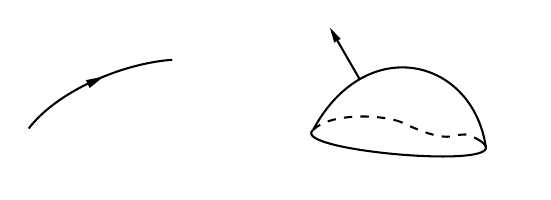
\begin{tikzpicture}[x=0.75pt,y=0.75pt,yscale=1,xscale=1]
%uncomment if require: \path (0,300); %set diagram left start at 0, and has height of 300

%Curve Lines [id:da7826517172347827] 
\draw    (3.65,18.88) .. controls (17.2,36.58) and (48,50.16) .. (72.8,51.99) ;
\draw [shift={(39.71,43.88)}, rotate = 205.45] [fill={rgb, 255:red, 0; green, 0; blue, 0 }  ][line width=0.08]  [draw opacity=0] (8.4,-2.1) -- (0,0) -- (8.4,2.1) -- cycle    ;
%Curve Lines [id:da8566552148207576] 
\draw    (221.73,12.59) .. controls (241.17,-1.67) and (128.44,8) .. (140.66,18.19) ;
%Curve Lines [id:da14270801999584393] 
\draw  [dash pattern={on 3pt off 3pt on 3pt off 3pt}]  (183.2,21.91) .. controls (174,25.58) and (149.2,26.68) .. (140.66,18.19) ;
%Curve Lines [id:da5926224666835718] 
\draw  [dash pattern={on 3pt off 3pt on 3pt off 3pt}]  (221.73,12.59) .. controls (206.74,22.26) and (214.4,6.87) .. (183.2,21.91) ;
%Curve Lines [id:da4918795365326445] 
\draw    (223.95,9.53) .. controls (217.84,52.82) and (166.2,65.55) .. (140.66,18.19) ;
%Straight Lines [id:da406966878688231] 
\draw    (163.2,42.45) -- (149.8,65.67) ;
\draw [shift={(148.8,67.4)}, rotate = 299.99] [fill={rgb, 255:red, 0; green, 0; blue, 0 }  ][line width=0.08]  [draw opacity=0] (7.2,-1.8) -- (0,0) -- (7.2,1.8) -- cycle    ;

\end{tikzpicture}
    \caption{曲线、曲面的定向}
\end{figure}

\section{带边流形}

现借助坐标系叙述之。在 $M$ 中有一包含 $p$ 的局部坐标系 $(O,\psi;x^i)$,使得 $\psi(p)$ 是坐标原点且 $U\cap D =\{q\in U|x^1(q)\leqslant 0\}$,则称 $D$ 是 $M$ 上的一个\textit{带边区域},其边界点 $x^1$ 坐标为零。坐标空间里这个区域就称作“\textit{半空间(half-space)}” $\mathbb H^{n}$,有时可记作 $\frac{1}{2}\R^n$。由于边界点失去了一个坐标自由度,因此我们很容易发现 $\partial D$ 是相较于 $D$ 而言“余 1 维(1-codimension)”。考虑到背景和内部都是同维开集,因此说\textit{带边区域不能直接认同为普通开集},因其在实质上“强行”拼凑了两个不同维度的东西,即内部和边界。

区域定向可在其边界上也诱导出与之相应的定向

\begin{figure}[h!]
    \centering
\tikzset{
pattern size/.store in=\mcSize, 
pattern size = 5pt,
pattern thickness/.store in=\mcThickness, 
pattern thickness = 0.3pt,
pattern radius/.store in=\mcRadius, 
pattern radius = 1pt}
\makeatletter
\pgfutil@ifundefined{pgf@pattern@name@_hask52a3i}{
\pgfdeclarepatternformonly[\mcThickness,\mcSize]{_hask52a3i}
{\pgfqpoint{0pt}{0pt}}
{\pgfpoint{\mcSize+\mcThickness}{\mcSize+\mcThickness}}
{\pgfpoint{\mcSize}{\mcSize}}
{
\pgfsetcolor{\tikz@pattern@color}
\pgfsetlinewidth{\mcThickness}
\pgfpathmoveto{\pgfqpoint{0pt}{0pt}}
\pgfpathlineto{\pgfpoint{\mcSize+\mcThickness}{\mcSize+\mcThickness}}
\pgfusepath{stroke}
}}
\makeatother

% Pattern Info
 
\tikzset{
pattern size/.store in=\mcSize, 
pattern size = 5pt,
pattern thickness/.store in=\mcThickness, 
pattern thickness = 0.3pt,
pattern radius/.store in=\mcRadius, 
pattern radius = 1pt}
\makeatletter
\pgfutil@ifundefined{pgf@pattern@name@_9v4tzcn4d}{
\pgfdeclarepatternformonly[\mcThickness,\mcSize]{_9v4tzcn4d}
{\pgfqpoint{0pt}{0pt}}
{\pgfpoint{\mcSize+\mcThickness}{\mcSize+\mcThickness}}
{\pgfpoint{\mcSize}{\mcSize}}
{
\pgfsetcolor{\tikz@pattern@color}
\pgfsetlinewidth{\mcThickness}
\pgfpathmoveto{\pgfqpoint{0pt}{0pt}}
\pgfpathlineto{\pgfpoint{\mcSize+\mcThickness}{\mcSize+\mcThickness}}
\pgfusepath{stroke}
}}
\makeatother
\tikzset{every picture/.style={line width=0.75pt}} %set default line width to 0.75pt        

\begin{tikzpicture}[x=0.75pt,y=0.75pt,yscale=1,xscale=1]
%uncomment if require: \path (0,300); %set diagram left start at 0, and has height of 300

%Shape: Polygon Curved [id:ds6324304927731197] 
\draw   (14,85) .. controls (10,122) and (65.25,88.75) .. (74.25,80.25) .. controls (83.25,71.75) and (88.25,58.25) .. (81.25,45.25) .. controls (74.25,32.25) and (36.25,-5.25) .. (16.25,24.75) .. controls (-3.75,54.75) and (18,48) .. (14,85) -- cycle ;
%Shape: Rectangle [id:dp42790425123431874] 
\draw  [dash pattern={on 4.5pt off 4.5pt}] (142,117) node[below right]{$\mathbb H^n$} -- (252,117)node[below right]{$\R^n$} -- (252,7) -- (142,7) -- cycle ;
%Straight Lines [id:da2780621449052143] 
\draw    (197,117) -- (197,7) ;
%Curve Lines [id:da11211326883897499] 
\draw [pattern=_hask52a3i,pattern size=6pt,pattern thickness=0.75pt,pattern radius=0pt, pattern color={rgb, 255:red, 0; green, 0; blue, 0}] [dash pattern={on 4.5pt off 4.5pt}]  (197,25) .. controls (167,52) and (161,80) .. (196,97) ;
%Shape: Polygon Curved [id:ds6020575675206878] 
\draw  [pattern=_9v4tzcn4d,pattern size=6pt,pattern thickness=0.75pt,pattern radius=0pt, pattern color={rgb, 255:red, 0; green, 0; blue, 0}][dash pattern={on 4.5pt off 4.5pt}] (57.25,56.75) .. controls (55.75,74.75) and (65.25,88.75) .. (74.25,80.25) .. controls (83.25,71.75) and (88.25,58.25) .. (81.25,45.25) .. controls (74.25,32.25) and (58.75,38.75) .. (57.25,56.75) -- cycle ;
%Curve Lines [id:da8087172400108391] 
\draw [line width=0.75]    (77.25,67.75) .. controls (119.39,104.75) and (169.21,96.84) .. (192.37,74.39) node[near start,sloped,above]{$\psi$};
\draw [shift={(193.75,73)}, rotate = 133.75] [fill={rgb, 255:red, 0; green, 0; blue, 0 }  ][line width=0.08]  [draw opacity=0] (8.4,-2.1) -- (0,0) -- (8.4,2.1) -- cycle    ;
\end{tikzpicture}
    \caption{带边区域}
\end{figure}

\section{超曲面}


\begin{definition}[切矢和法矢]
    设 $S$ 是背景 $M$ 上可具有不同维度的子集。将 $S$ 上一点 $q$ 处的矢量称为切矢 $w$,若 $S$ 上存在过 $q$ 的曲线与其相切。用坐标基易验证,$q$ 处所有矢量构成的矢量空间 $V_q$ 与 $M$ 同维,而所有 $w$ 所构成的集合称作切空间,记作 $T_q S$,是 $V_q$ 的矢量子空间。

    可以定义 $q$ 处的法矢 $n$,若对任意切矢 $w$ 有 $\langle n,w\rangle=0$,这里内积取决于 $M$ 所选度规。
\end{definition}
\begin{theorem}
    当 $S$ 是 $M$ 的余 1 维子空间时,又可以形象地叫做一张,其上一点的任意法矢间只差倍数关系。
\end{theorem}


\begin{proof}
    证明 设 $\left\{e_2, \cdots,e_n\right\}$ 为 $T_q S$ 任一坐标基, 因 $\dim V_q=n, V_q$ 必有与 $\left\{e_2,\cdots,e_n\right\}$ 线性无关的元素, 任取其一并记作 $e_1$, 则 $\left\{e_\mu\mid\mu=1, \cdots, n\right\}$ 为 $V_q$ 的基底。令 $n=e_1$, 则 $\langle n, e_\tau\rangle =g(e_1,e_\tau)=0$,这里 $\tau=2,\cdots,n$,可见 $n$ 为法矢。若存在 $m$ 满足 $\langle m,e_\tau\rangle=0$, 则其在 $\left\{e_\mu\right\}$ 的分量 $m^\tau=0$, 因而只剩下分量 $m^1$,即 $m=m^1\left(e_1\right)^a$ $=m^1n$, 即 $m$ 与 $n$ 只差一因子 $m^1$。
\end{proof}

注意,余维数太多的话,比如三维空间的曲线,其上法矢就没有该性质了,因此选取更为任意。对于超曲面,约定其模长可以使得差别仅体现在“内外方向”上。以后默认取单位法矢,即要求 $\langle n,n\rangle=\pm 1$,正负号来自度规的正负定性。设 $p\in S$ 上的一个局部坐标系 $(U;x^1,\cdots,x^{n})$ 是 $M$ 正定的右手系使得域内点 $x^n\leqslant 0$,则$(U\cap S;x^1,\cdots,x^{n-1})$ 也是 $S$ 的局部坐标系,且 $\pdv{x^n}$ 就是法矢而且是外法矢。

对一点 $q$,度规的作用范围是其整个矢量空间 $V_q$,因此类似于切矢,度规也有“切于” $S$ 的部分,那就是只作用于 $T_qS$ 的部分。


此外,任意 $l$-形式也能按相应思路定义其\textbf{诱导形式},这是有必要的,因为一旦把 $S$ 看作一个独立区域,而非从背景的嵌入视角观察,那么“不切于”的形式都是没有意义的。
体元、定向也是形式,自然也有其诱导。


